\documentclass{article}
\usepackage[utf8]{inputenc}
\usepackage[T1]{fontenc}
\usepackage[table,xcdraw]{xcolor}
\usepackage{float}
\usepackage{tabularx}
\usepackage{amsmath}
\usepackage{url}
\usepackage{booktabs}
\usepackage{graphicx}
\usepackage[english,polish]{babel}

\title{Analiza zmian statystyk ligi NBA od początku lat 90-tych oraz ich porównanie}
\author{Kacper Balbus}
\date{\today}

\begin{document}

\maketitle

\newpage
\vspace{4cm}


\tableofcontents
\newpage

\section{Wstęp}



Liga NBA (National Basketball Association) jest najbardziej rozpoznawalną i oglądaną ligą koszykówki na całym świecie. Od początku lat 90-tych do dziś, przeszła ona wiele zmian, zarówno pod względem stylu gry, jak i statystyk osiąganych przez zawodników. Coraz częściej pojawiają się opinie sugerujące, że liga zmierza w złym kierunku, jej poziom się obniżył, a jej "złotymi czasami" były właśnie lata 90-te. Zestawienie i analiza wszytskich danych, powinna w widoczny sposób przedstawić nam, gdzie najbardziej widać różnicę teraźniejszości względem lat 90-tych oraz czy rzeczywiście, w tamtych czasach, na boiskach NBA panował wyższy poziom. Celem projektu jest zbadanie, jak zmieniały się poszczególne statystyki od sezonu 1990-91 do sezonu 2022-23, znalezienie korelacji pomiędzy poszczególnymi statystykami, stworzenie modelu, który umożliwi określenie czy drużyna osiągająca konkretne statystyki, w podanym sezonie zasadniczym, byłaby w stanie dostać się do fazy play-off oraz przy jego pomocy sprawdzenie, jak poradziłyby sobie drużyny, gdyby osiągnęły konkretne statystyki w podanym sezonie. Naszym głównym narzędziem do odczytywania danych oraz pracy na nich, będzie Python.


\section{Słownik}
\begin{itemize}
    \item FG (Field goals) - liczba udanych rzutów.
    \item 3P (3 pointers) - liczba udanych rzutów za 3 punkty.
    \item FT (Free throws) - liczba udanych rzutów osobistych.
    \item TRB (Total rebounds) - liczba udanych zbiórek w ataku i obronie.
    \item AST (Assists) - liczba asyst.
    \item STL (Steals) - liczba odbiorów.
    \item BLK (Blocks) - liczba bloków.
    \item TOV (Turnovers) - liczba strat.
    \item PF (Personal fouls) - liczba popełnionych fauli.
    \item PTS (Points) - liczba punktów.
\end{itemize}


\section{Zbiór danych i jego przetwarzanie}

\subsection{Zbiór danych}
    
Do rozwiązania problemu skorzystałem ze zbiorów danych dostępnych na stronie internetowej basketball-reference.com:
\begin{enumerate}
    \item Zbiór "NBA League Averages - Per Game" zawiera dane średnich statystyk całej ligi, w jednym meczu, w każdym sezonie od 1990-91. Posłuży on do obserwacji zmian poszczególnych statystyk na przestrzeni lat oraz znalezienia korelacji pomiędzy nimi.
    \item Zbiory "Per Game Stats" (jeden zbiór dotyczy jednego sezonu) zawierają średnie statystyki każdej drużyny, z sezonu zasadniczego, na jeden mecz oraz informację, czy dana drużyna dostała się do fazy play-off. Te zbiory zostaną przez nas wykorzystane do opracowania modelu i wykonania na nim eksperymentów.
\end{enumerate}


\subsection{Przetwarzanie wstępne}
\begin{enumerate}
    \item Ze zbioru "NBA League Averages - Per Game", korzystając z programu Excel, usunięto niepotrzebne kolmuny danych. Po zmianach zawiera on kolumnę określającą sezon, z którego pochodzi wiersz oraz kolumny zawierające średnie statystyki wymienione w słowniku.
    \item Zbiory "Per Game Stats" zostały połączone w jeden zbiór, zawierajacy średnie statystyki drużyn z każdego sezonu od 1990-91. Korzystając z programu Excel dodane zostały dwie dodatkowe kolumny:
    \begin{itemize}
        \item Season - określająca z jakiego sezonu pochodzi konkretny wiersz.
        \item Playoffs - określająca, binarnie  ("YES" lub "NO"), czy dana drużyna dostała się do fazy play-off. Wcześniej określane to było w kolumnie Team i symbolizowane było gwiazdką występującą po nazwie zaspołu.
    \end{itemize}
    Następnie usunięto niepotrzebne kolumny danych, aby pozostały jedynie wcześniej stworzone oraz zawierające średnie statystyki wymienione w słowniku.
\end{enumerate}

\subsection{Przykładowe dane}
\begin{enumerate}
    \item "NBA League Averages - Per Game"
        \begin{table}[H]
            \centering
            \begin{tabular}{|l|l|l|l|l|l|l|l|l|l|l|}
            \hline
            \textbf{Season} & \textbf{FG} & \textbf{3P} & \textbf{FT} & \textbf{TRB} & \textbf{AST} & \textbf{STL} & \textbf{BLK} & \textbf{TOV} & \textbf{PF} & \textbf{PTS} \\ \hline
            2022-23 & 42.0 & 12.3 & 18.4 & 43.4 & 25.3 & 7.3 & 4.7 & 14.1 & 20.0 & 114.7 \\ \hline
            2021-22 & 40.6 & 12.4 & 16.9 & 44.5 & 24.6 & 7.6 & 4.7 & 13.8 & 19.6 & 110.6 \\ \hline
            2020-21 & 41.2 & 12.7 & 17.0 & 44.3 & 24.8 & 7.6 & 4.9 & 13.8 & 19.3 & 112.1 \\ \hline
            \end{tabular}
        \end{table}
    \item "Per Game Stats"
        \begin{table}[H]
            \centering
            \begin{tabular}{|l|l|l|l|l|l|l|l|l|l|l|l|}
            \hline
            \textbf{Season} & \textbf{FG} & \textbf{3P} & \textbf{FT} & \textbf{TRB} & \textbf{AST} & \textbf{STL} & \textbf{BLK} & \textbf{TOV} & \textbf{PF} & \textbf{PTS} & \textbf{Playoffs} \\ \hline
            2022-23 & 43.6 & 13.8 & 19.8 & 42.5 & 27.3 & 7.0 & 3.4 & 13.5 & 19.7 & 120.7 & YES \\ \hline
            2022-23 & 42.0 & 13.6 & 18.7 & 41.5 & 27.0 & 7.7 & 5.8 & 14.9 & 21.2 & 116.3 & NO \\ \hline
            2002-03 & 32.8 & 2.8 & 15.8 & 42.4 & 21.2 & 8.7 & 5.1 & 18.5 & 25.1 & 84.2 & NO \\ \hline
            \end{tabular}
        \end{table}
\end{enumerate}

\newpage

\section{Ekspolracja danych}

    \subsection{Zmiany statystyk na przestrzeni sezonów}
    
    \begin{enumerate}
        \item Liczba trafionych rzutów:
            \begin{figure}[H]
                \centering
                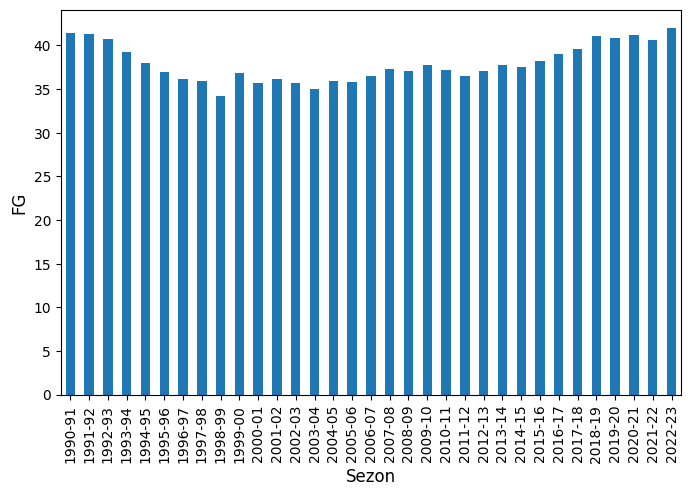
\includegraphics[width=10cm]{wykres_FG.png}
                \caption{Średnia liczba trafionych rzutów na mecz na przestrzeni sezonów}
                \label{fig:wykres_FG}
            \end{figure}

        Statystyka w latach 90-tych spadła o 5 i utrzymywała się w okolicy 35 trafionych rzutów na mecz. Od sezonu 2006-07 statystyka znów zaczęła się zwiększać i w obecnym sezonie znów wyniosła więcej niż 40.

  \newpage
        \item Liczba trafionych rzutów za 3 punkty:
            \begin{figure}[H]
                \centering
                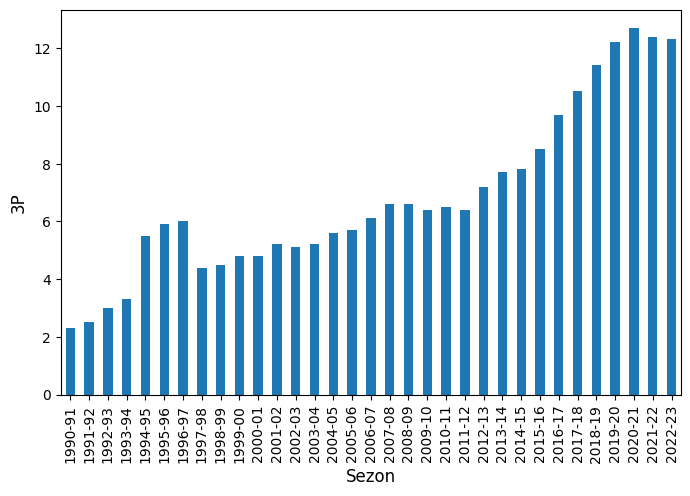
\includegraphics[width=10cm]{wykres_3P.png}
                \caption{Średnia liczba trafionych rzutów za 3 punkty na mecz na przestrzeni sezonów}
                \label{fig:wykres_3P}
            \end{figure}

        Od sezonu 1990-91 wzrosła ona sześciokrotnie osiągając w ostatnich 4 sezonach okolice 12 na mecz. Najbardziej gwałtowny wzrost wystąpił od sezonu 2011-12 i wyniósł 6. Warto również zwrócić uwagę na sezony od 1994-95 do 1996-97, które widocznie wyróżniają się w porównaniu z innymi sezonami w latach 90-tych, mając prawie dwukrotnie większą średnią punktów. Było to skutkiem tymczasowgo skróceniem, w tych sezonach, odległości linii rzutu za 3 punkty.
 \newpage         
        \item Liczba trafionych rzutów osobistych:
            \begin{figure}[H]
                \centering
                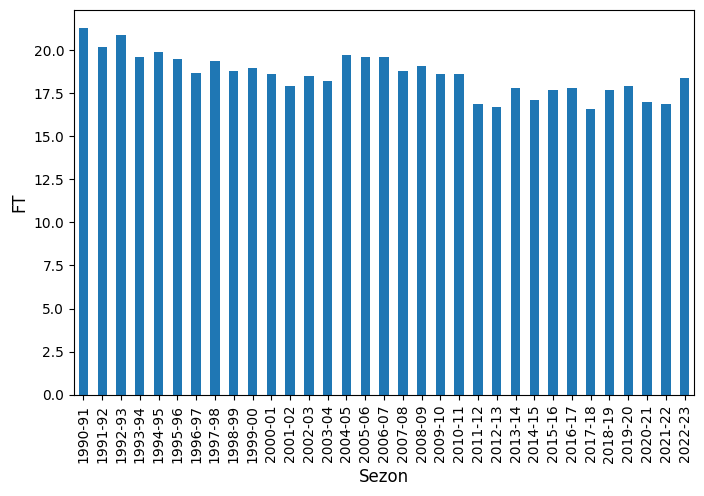
\includegraphics[width=10cm]{wykres_FT.png}
                \caption{Średnia liczba trafionych osobistych na mecz na przestrzeni sezonów}
                \label{fig:wykres_FT}
            \end{figure}

        Średnia liczba trafianych rzutów osobistych spadła z około 21 w sezonie 1990-91 do 17.5 w sezonie 2003-04, następnie w sezonach od 2004-05 do 2010-11 ponownie wynosiła około 19. Od sezonu 2011-12 wynosiła najmniej, bo utrzymywała się w okolicy 17.5 na mecz.
 \newpage            
        \item Liczba zbiórek:
            \begin{figure}[H]
                \centering
                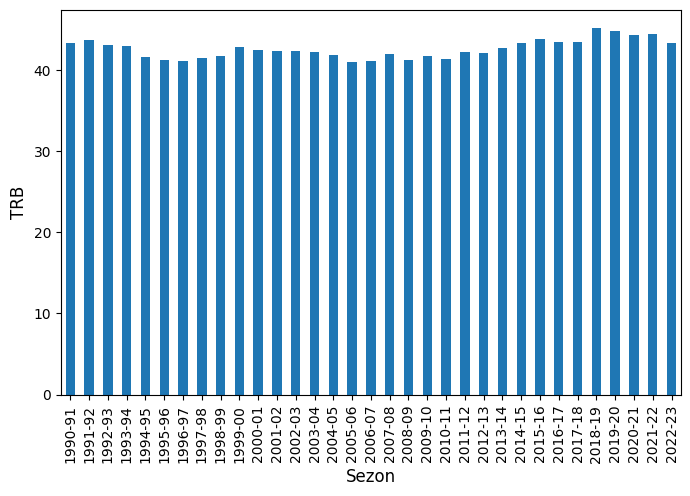
\includegraphics[width=10cm]{wykres_TRB.png}
                \caption{Średnia liczba zbiórek na mecz na przestrzeni sezonów}
                \label{fig:wykres_TRB}
            \end{figure}

        Liczba zbiórek zanotowała nieznaczny spadek o 2 na początku lat 90-tych, finalnie wracając w sezonie 2013-14 do początkowego poziomu 43 zbiórek na mecz.
 \newpage        
        \item Liczba asyst:
            \begin{figure}[H]
                \centering
                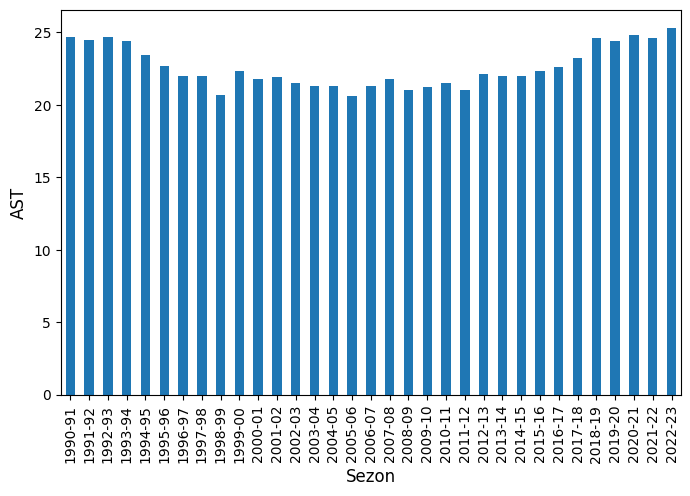
\includegraphics[width=10cm]{wykres_AST.png}
                \caption{Średnia liczba asyst na mecz na przestrzeni sezonów}
                \label{fig:wykres_AST}
            \end{figure}


        Liczba asyst zanotowała w latach 90-tych znaczny spadek, bo aż o 5, następnie utrzymywała się w okolicach 20, aby ponownie od sezonu 2012-13 wzrosnąć do 25, czyli nieco powyżej liczby z sezonu 1990-91.
  \newpage           
        \item Liczba odbiorów:
            \begin{figure}[H]
                \centering
                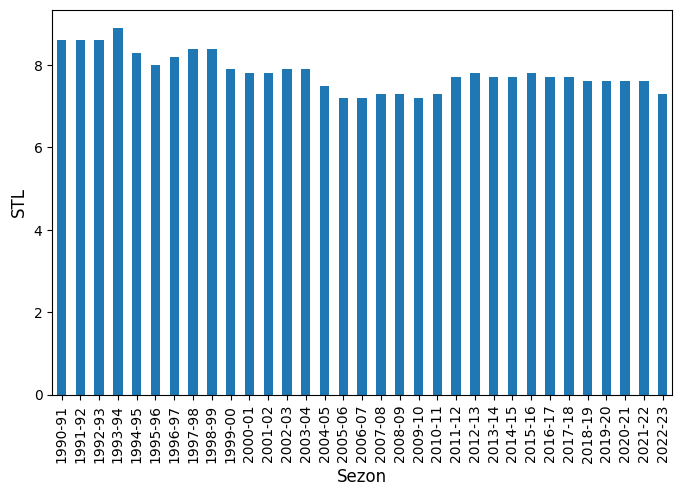
\includegraphics[width=10cm]{wykres_STL.png}
                \caption{Średnia liczba odbiorów na mecz na przestrzeni sezonów}
                \label{fig:wykres_STL}
            \end{figure}

        Liczba odbiorów sukcesywnie zmiejszała się od połowy lat 2000-nych z 8.5 do 7.5. Od sezonu 2011-12 liczba ta minimalnie wzrosła do 8 i utrzymywała się na podobnym poziomie.
 \newpage         
        \item Liczba bloków:
            \begin{figure}[H]
                \centering
                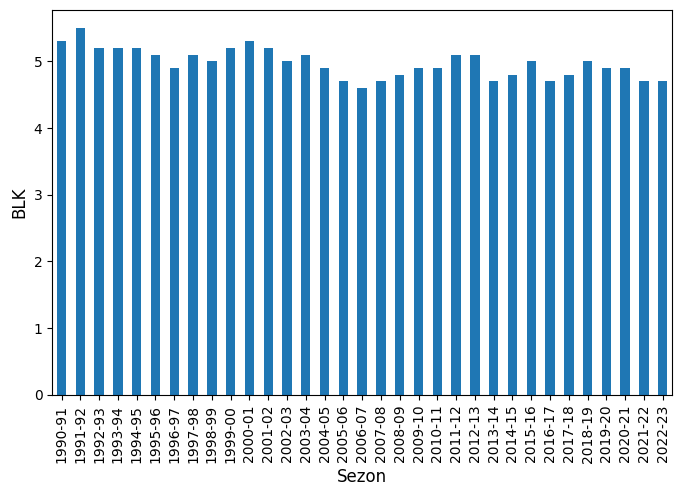
\includegraphics[width=10cm]{wykres_BLK.png}
                \caption{Średnia liczba bloków na mecz na przestrzeni sezonów}
                \label{fig:wykres_BLK}
            \end{figure}

        Liczba bloków nie zanotowała znaczących zmian, notując wzrosty i spadki na przestrzeni analizowanych seoznów, ostatecznie zmniejszajać się o 0.5 w porównaniu do sezonów na początku lat 90-tych.
 \newpage            
        \item Liczba strat:
            \begin{figure}[H]
                \centering
                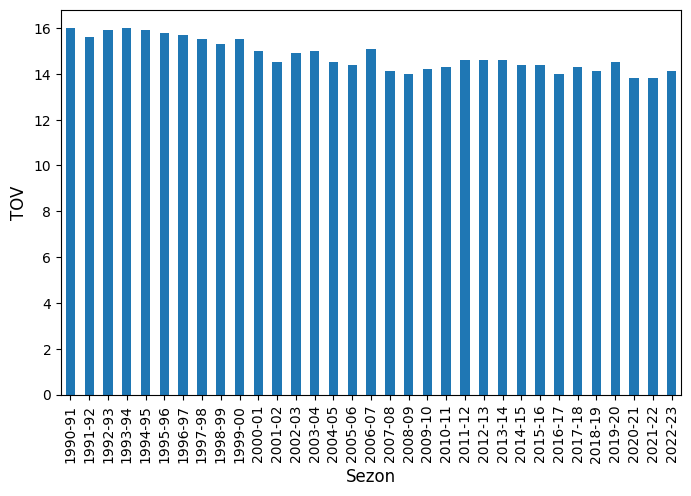
\includegraphics[width=10cm]{wykres_TOV.png}
                \caption{Średnia liczba strat na mecz na przestrzeni sezonów}
                \label{fig:wykres_TOV}
            \end{figure}

        Liczba strat konsekwentnie zmniejszała się z seoznu na sezon, finalnie notując spadek o 2 w porównaniu do wartości początkowej.
\newpage             
        \item Liczba popełnionych fauli:
            \begin{figure}[H]
                \centering
                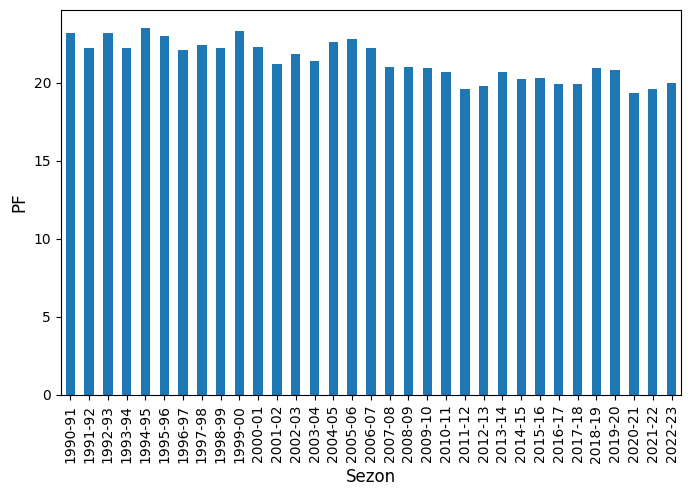
\includegraphics[width=10cm]{wykres_PF.png}
                \caption{Średnia liczba popełnionych fauli na mecz na przestrzeni sezonów}
                \label{fig:wykres_PF}
            \end{figure}

        Statystyka popełnionych fauli wzrastała i zmniejszała się z sezonu na   sezon, finalnie notując spadek wynoszący około 3 na mecz.
\newpage         
        \item Liczba punktów:
            \begin{figure}[H]
                \centering
                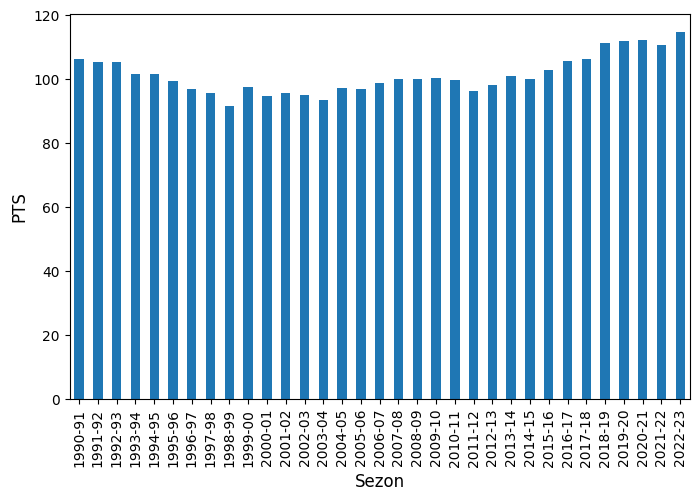
\includegraphics[width=10cm]{wykres_PTS.png}
                \caption{Średnia liczba punktów na mecz na przestrzeni sezonów}
                \label{fig:wykres_PTS}
            \end{figure}
            
        Liczba punktów spadała gwałtownie z każdym sezonem od 1990-91 do 1998-99, zminiejszjąc się, aż o 15. Potem jednak trend się odwrócił i trwa aż do dziś, skutkując dotychczasowym wzrostem z 91.5 na 114.7.
            
        \item Podsumowanie
        
    Wykresy przygotowane zostały korzystając z biblioteki matplotlib.
    
    Warto zauważyć, że statystyki zmieniały się na 3 sposoby:
    \begin{itemize}
        \item Spadek (FT, STL, BLK, TOV, PF)
        \item Spadek, a następnie wzrost (FG, TRB, AST, PTS)
        \item Wzrost (3P)
    \end{itemize}

    Jedyną statystyką, która konsekwentnie zwiększała się jest liczba udanych rzutów za 3 punkty. Jest to również statystyka notująca największą różnicę w porównaniu do sezonu 1990-91, ponieważ jej aktualna wartość jest prawie 6-krotnie większa. Najwięcej statystyk zaliczyło spadek (5). Jednak każda ze zmniejszających się statystyk zmniejszyła się tylko nieznacznie. Cechą wspólną statystyk notujących spadek, a następnie wzrost jest fakt, że spadek występował w każdym przypadku na przestrzeni lat 90-tych, następnie utrzymując się na podobnym poziomie do późnych lat 2000-nych lub początku lat 2010-tych, aby ponownie wzrosnąć do wartości osiąganych na początku lat 90-tych, a nawet je przekraczając.

    \end{enumerate}

    \subsection{Zależności między statystykami}

    Mapa korelacji stworzona została, korzystając z biblioteki seaborn.

    Jako wartości mocno skorelowane zostały uznane wszystkie związki, posiadające współczynnik korelacji wynoszący  powyżej 0.65 lub poniżej -0.65.
    
        \begin{figure}[H]
            \centering
            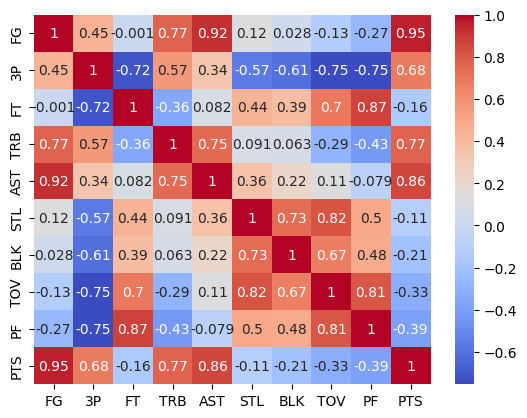
\includegraphics[width=10cm]{mapa_korelacji.png}
            \caption{Mapa korelacji średnich statystyk}
            \label{fig:mapa_korelacji}
        \end{figure}
    
    Powyższa mapa korelacji wykazuje silny wpływ wielu statystyk na siebie. Najwięcej mocnych zależności, wykazuje średnia liczba punktów na mecz oraz liczba udanych rzutów za 3 punkty (4). Liczba punktów jest statystyką rozstrzygająca wynik meczu, co powoduje, że wpływa na nią największa ilość innych statystyk. Można spostrzec, że poza statystykami ewidentnie ofensywnymi, duży wpływ ma na nią również liczba zbiórek, czyli statystyka, bardziej defensywna niż ofensywna. Duża ilość silnych korelacji liczby rzutów za 3 punkty, najprawdopodobniej związana jest z faktem, że jest to statystyka, która zmieniała się najbardziej. Była to również jedyna statystyka posiadająca więcej niż 1 mocną korelaję ujemną, co najprawdopodobniej spowodowane jest jej konsekwentnym wzrostem, przy spadku aż 5 statystyk. Najmocniej korelują ze sobą dwie grupy statystyk: FG, AST, TRB, PTS oraz STL, TOV, BLK.
\newpage
    \subsection{Analiza zależności między statystykami}

    Każdy z dopasowanych trendów został obliczony korzystając z metody najmniejszych kwadratów i wykorzystując algorytm analityczny:

    \begin{equation}
    \hat{\theta} = (X X^T)^{-1} X Y^T
    \end{equation}

    Przy obliczeniach i wizualizacji wykresów wykorzystano biblioteki pandas, numpy oraz matplotlib.
    
    \begin{enumerate}
        \item Wpływ liczby zbiórek na liczbę udanych rzutów:
        
        
        Trend:\begin{equation} y = 1.466x - 24.542 \end{equation}
        
            \begin{figure}[H]
                \centering
                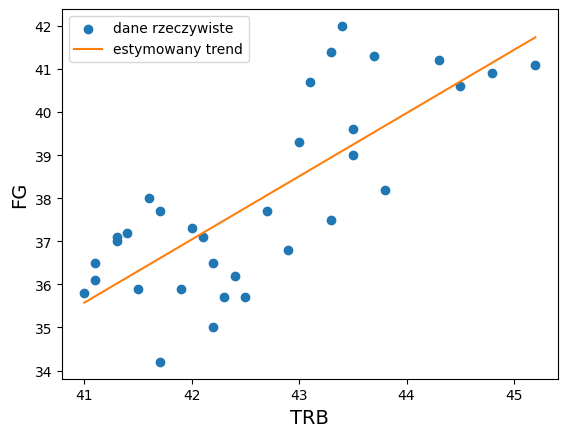
\includegraphics[width=10cm]{wykres_zaleznosci_FG_od_TRB.png}
                \caption{Zależność liczby udanych rzutów od liczby zbiórek}
                \label{fig:wykres_zaleznosci_FG_od_TRB}
            \end{figure}

        Liczba zbiórek liniowo wpływa na liczbę udanych rzutów. Im więcej piłek uda się zebrać drużynie, tym więcej może oddać rzutów, co prowadzi do większej ilości rzutów udanych.    
 \newpage            
        \item Wpływ liczby udanych rzutów na liczbę asyst:
        
        
        Trend:\begin{equation} y = 0.61x - 0.56 \end{equation}
        
            \begin{figure}[H]
                \centering
                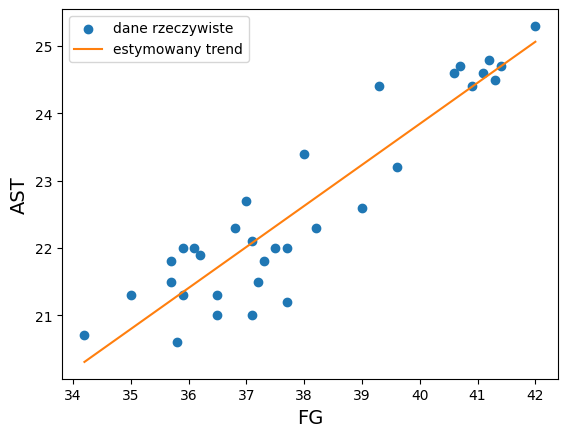
\includegraphics[width=10cm]{wykres_zaleznosci_AST_od_FG.png}
                \caption{Zależność liczby asyst od liczby udanych rzutów}
                \label{fig:wykres_zaleznosci_AST_od_FG}
            \end{figure}

        Większa liczba udanych rzutów bezpośrednio powoduje, że większa liczba rzutów po podaniach, również jest udana, co prowadzi do większej liczby asyst.
  \newpage       
        \item Wpływ liczby udanych rzutów na liczbę punktów:
        
        
        Trend:\begin{equation} y = 2.597x + 2.761 \end{equation}
        
            \begin{figure}[H]
                \centering
                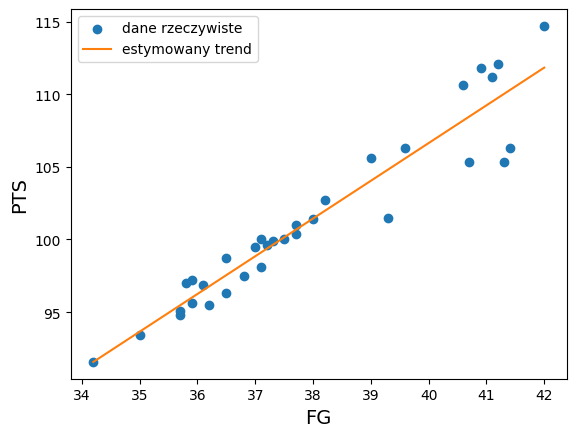
\includegraphics[width=10cm]{wykres_zaleznosci_PTS_od_FG.png}
                \caption{Zależność liczby punktów od liczby udanych rzutów}
                \label{fig:wykres_zaleznosci_PTS_od_FG}
            \end{figure}


        Jest to najmocniejsza korelacja statystyk. Liczba udanych rzutów bezpośrednio wpływa na liczbę punktów, gdyż liczba punktów jest na jej podstawie obliczana.
\newpage 
        \item Wpływ liczby udanych rzutów za 3 punkty na liczbę punktów:
        
        
        Trend:\begin{equation} y = 0.384x^{2} - 4.628x + 111.803 \end{equation}
        
            \begin{figure}[H]
                \centering
                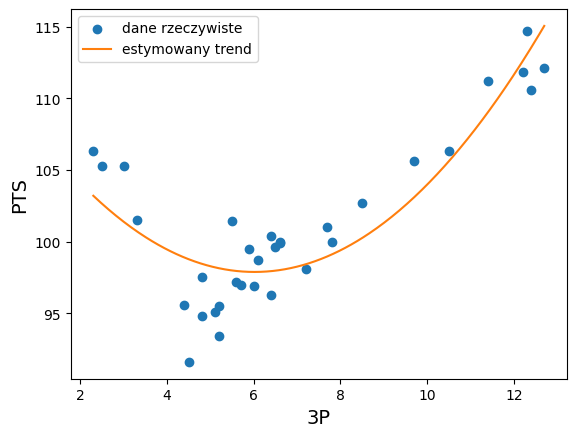
\includegraphics[width=10cm]{wykres_zaleznosci_PTS_od_3P.png}
                \caption{Zależność liczby punktów od liczby udanych rzutów za 3 punkty}
                \label{fig:wykres_zaleznosci_PTS_od_3P}
            \end{figure}

        Najlepiej dopasowanym trendem do tej korelacji jest trend kwadratowy. Liczba punktów maleje wraz ze wzrostem liczby udanych rzutów za 3 punkty na przedziale od 0 do 5.5, natomiast od tego momentu już tylko wzrasta. Oznacza to, że gdy gracze oddają mało udanych rzutów za 3 punkty, zdobywają lepszy wynik, rzucając w inny sposób, natomiast gdy liczba ich udanych rzutów za 3 punkty zaczyna przekraczać 8, znacząco zwiększa to ich sumaryczna liczba punktów na mecz. Przewidywana liczba punktów na mecz, przy braku udanych rzutów za 3 punkty (112), przekraczana jest przy zdobyciu 10 "trójek". Najgorsza liczba punktów osiągana była przy średniej wynoszącej 6 udanych rzutów za 3 punkty.    
\newpage 
        \item Wpływ liczby strat na liczbę udanych rzutów osobistych:
        
        
        Trend:\begin{equation} y = 1.184x - 1.05 \end{equation}
        
            \begin{figure}[H]
                \centering
                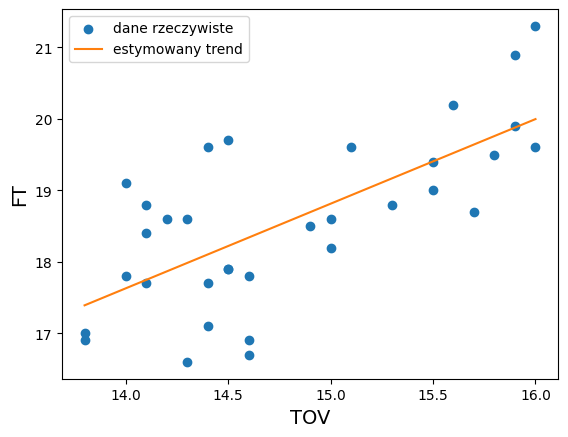
\includegraphics[width=10cm]{wykres_zaleznosci_FT_od_TOV.png}
                \caption{Zależność liczby udanych rzutów osobistych od liczby strat}
                \label{fig:wykres_zaleznosci_FT_od_TOV}
            \end{figure}


        Liczba udanych rzutów osobistych idzie liniowo w parze ze stratami. Straty często wynikają z prób zakłóceń przez drużynę przeciwną rzutu, co w wielu przypadkach skutkuje rzutami osobistymi.    
\newpage 
        \item Wpływ liczby popełnionych fauli na liczbę udanych rzutów osobistych:
        
        
        Trend:\begin{equation} y = 0.828x + 0.856 \end{equation}
        
            \begin{figure}[H]
                \centering
                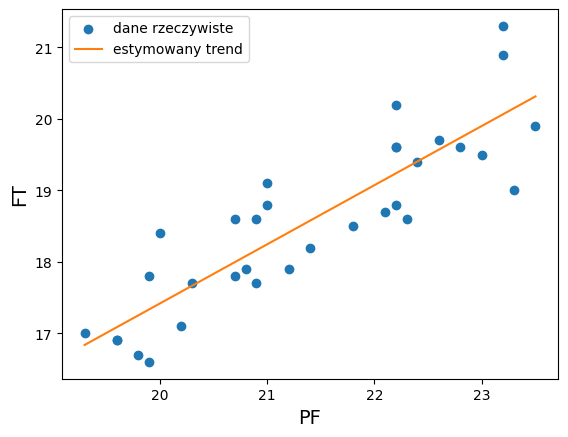
\includegraphics[width=10cm]{wykres_zaleznosci_FT_od_PF.png}
                \caption{Zależność liczby udanych rzutów osobistych od liczby popełnionych fauli}
                \label{fig:wykres_zaleznosci_FT_od_PF}
            \end{figure}


        Większa tendencja do popełniania fauli, skutkuje większą liczbą udanych rzutów osobistych. Rzuty osobiste bezpośrednio przyznawane są po nieprzepisowej próbie zakłócenia rzutu, co jest faulem. Obie statystyki naturalnie z siebie wynikają.  
\newpage 
        \item Wpływ liczby zbiórek na liczbę asyst:
        
        
        Trend:\begin{equation} y = 0.941x - 17.516 \end{equation}
        
            \begin{figure}[H]
                \centering
                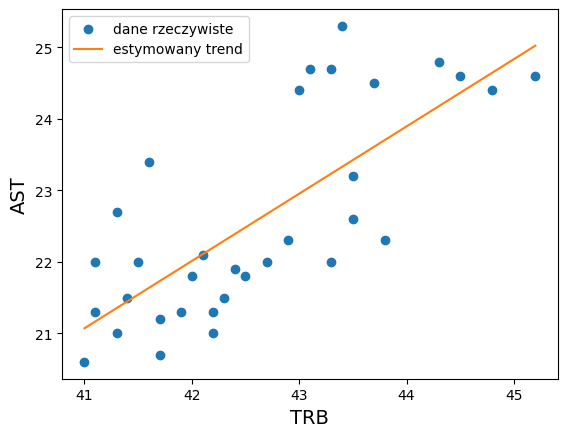
\includegraphics[width=10cm]{wykres_zaleznosci_AST_od_TRB.png}
                \caption{Zależność liczby asyst od liczby zbiórek}
                \label{fig:wykres_zaleznosci_AST_od_TRB}
            \end{figure}

        Większa liczba zbiórek prowadzi do większej ilości asyst, co powoduje występowanie trendu liniowego. Zbiórki bezpośrednio wpływają na możliwość dokonania podań, prowadzących do zdobycia punktów.
\newpage         
       \item Wpływ liczby zbiórek na liczbę punktów:
        
        
        Trend:\begin{equation} y = 3.995x - 68.947 \end{equation}
        
            \begin{figure}[H]
                \centering
                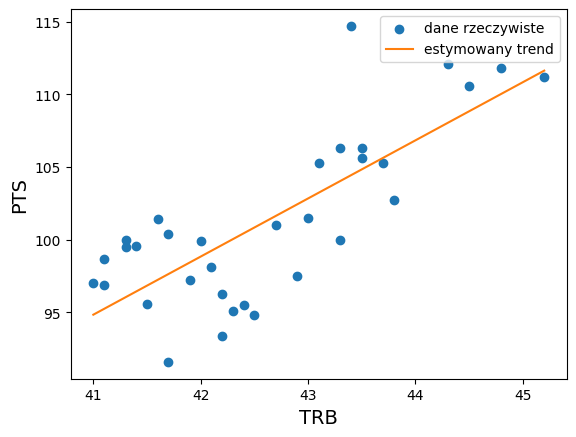
\includegraphics[width=10cm]{wykres_zaleznosci_PTS_od_TRB.png}
                \caption{Zależność liczby punktów od liczby zbiórek}
                \label{fig:wykres_zaleznosci_PTS_od_TRB}
            \end{figure}

        Większa liczba zbiórek, prowadzi liniowo, do większej liczby punktów. Podobnie jak w przypadku większej liczby udanych rzutów, zbiórki prowadzą do większej ilości okazji rzutowych, co przekłada się na liczbę punktów.
\newpage 
        \item Wpływ liczby asyst na liczbę punktów:
        
        
        Trend:\begin{equation} y = 3.534x + 21.469 \end{equation}
        
            \begin{figure}[H]
                \centering
                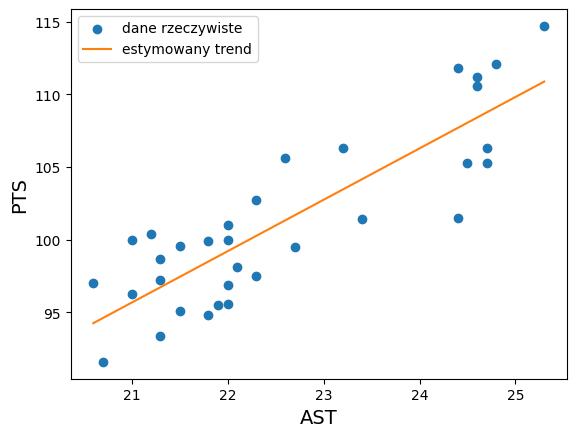
\includegraphics[width=10cm]{wykres_zaleznosci_PTS_od_AST.png}
                \caption{Zależność liczby punktów od liczby asyst}
                \label{fig:wykres_zaleznosci_PTS_od_AST}
            \end{figure}

        Asysty zaliczane są jedynie w przypadku, gdy zawodnik po podaniu zdobędzie punkt. Jest to więc naturalna zależność liniowa.
\newpage         
        \item Wpływ liczby strat na liczbę odbiorów:
        
        
        Trend:\begin{equation} y = 0.537x - 0.128 \end{equation}
        
            \begin{figure}[H]
                \centering
                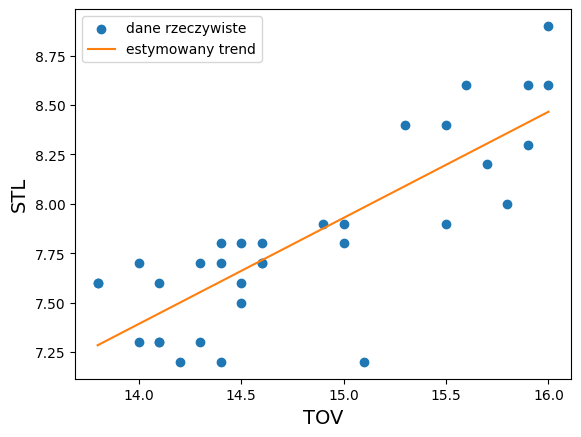
\includegraphics[width=10cm]{wykres_zaleznosci_STL_od_TOV.png}
                \caption{Zależność liczby odbiorów od liczby strat}
                \label{fig:wykres_zaleznosci_STL_od_TOV}
            \end{figure}


        Liczba strat obliczana jest na podstawie między innymi liczby odebranych piłek, przez drużynę przeciwną. W związku z tym, wymienione statystyki, są zależne od siebie liniowo.
\newpage 
        \item Wpływ liczby bloków na liczbę odbiorów:
        
        
        Trend:\begin{equation} y = 1.53x + 0.209 \end{equation}
        
            \begin{figure}[H]
                \centering
                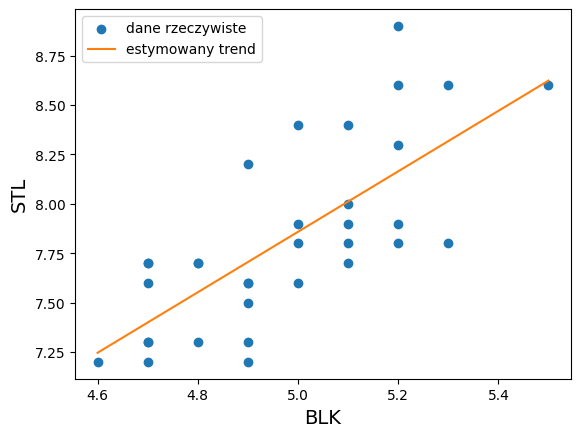
\includegraphics[width=10cm]{wykres_zaleznosci_STL_od_BLK.png}
                \caption{Zależność liczby odbiorów od liczby bloków}
                \label{fig:wykres_zaleznosci_STL_od_BLK.png}
            \end{figure}


        Liniowy wpływ wzrostu liczby bloków, na wzrost liczby odbiorów ukazuje, że statystyki defensywne, nawet pomimo braku bezpośredniego wpływu na siebie, są ze sobą mocno skorelowane.
\newpage 
        \item Wpływ liczby strat na liczbę bloków:
        
        
        Trend:\begin{equation} y = 0.209x + 1.881 \end{equation}
        
            \begin{figure}[H]
                \centering
                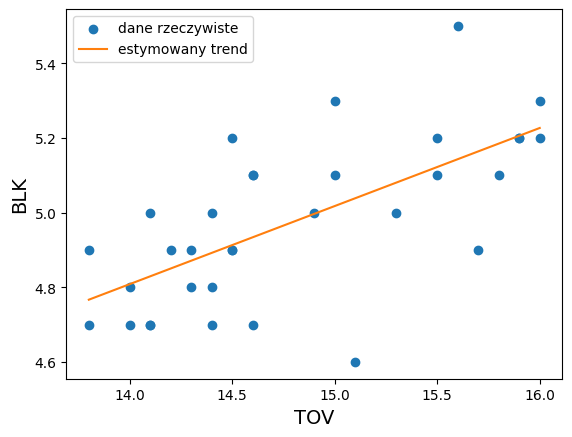
\includegraphics[width=10cm]{wykres_zaleznosci_BLK_od_TOV.png}
                \caption{Zależność liczby bloków od liczby strat}
                \label{fig:wykres_zaleznosci_BLK_od_TOV}
            \end{figure}

        Zwiększająca się liczba strat, daje drużynie przeciwnej więcej okazji do kontrataków, co prowadzi do zwiększenia się liczby bloków, które osiągnięte mogą zostać jedynie w defensywie.
\newpage 
        \item Wpływ liczby strat na liczbę popełnionych fauli:
        
        Trend:\begin{equation} y = 1.449x - 0.043 \end{equation}
        
        
            \begin{figure}[H]
                \centering
                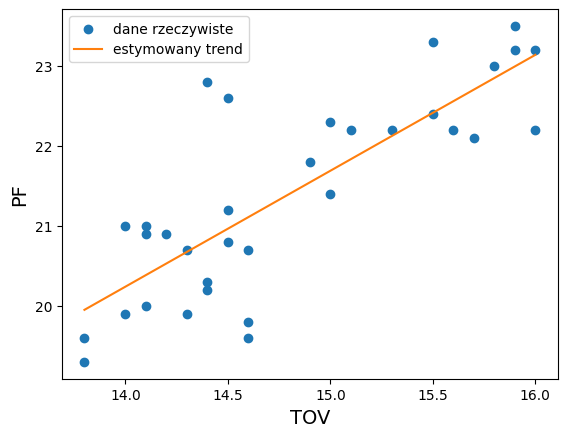
\includegraphics[width=10cm]{wykres_zaleznosci_PF_od_TOV.png}
                \caption{Zależność liczby popełnionych fauli od liczby strat}
                \label{fig:wykres_zaleznosci_PF_od_TOV}
            \end{figure}

        Wraz ze wzrostem liczby strat liniowo wzrasta liczba popełnionych fauli. Gracze mają tendencję do częstszego przekraczania przepisów, przy większej ilości prób wywołania straty u drużyny przeciwnej.  

        \newpage 
        \item Wpływ liczby udanych rzutów za 3 punkty na liczbę popełnionych fauli:
        
        Trend:\begin{equation} y = - 0.324x + 23.604 \end{equation}
        
            \begin{figure}[H]
                \centering
                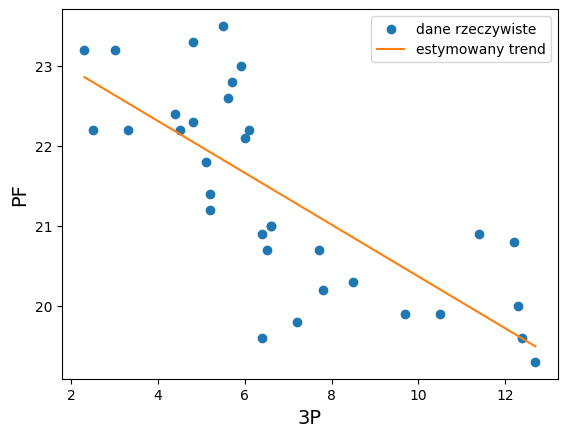
\includegraphics[width=10cm]{wykres_zaleznosci_PF_od_3P.png}
                \caption{Zależność liczby popełnionych fauli od liczby udanych rzutów za 3 punkty}
                \label{fig:wykres_zaleznosci_PF_od_3P}
            \end{figure}

        Wraz ze wzrostem liczby udanych rzutów za 3 punkty, liniowo maleje liczba popełnianych fauli. Jest to bezpośrednim wynikiem mniejszej potrzeby kontaktowej gry blisko kosza. 

        \newpage 
        \item Wpływ liczby udanych rzutów za 3 punkty na liczbę strat:
        
        
        Trend:\begin{equation} y = - 0.18x + 16.029 \end{equation}
        
            \begin{figure}[H]
                \centering
                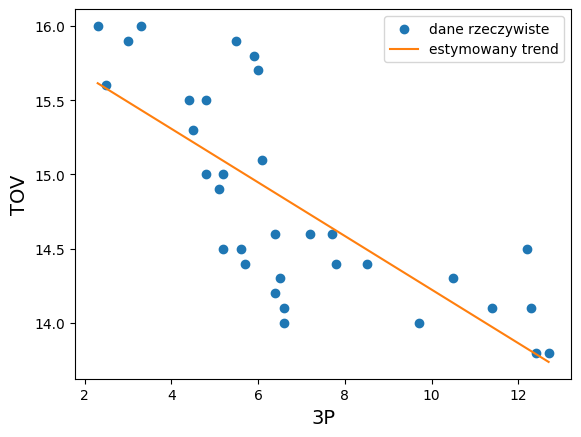
\includegraphics[width=10cm]{wykres_zaleznosci_TOV_od_3P.png}
                \caption{Zależność liczby strat od liczby udanych rzutów za 3 punkty}
                \label{fig:wykres_zaleznosci_TOV_od_3P}
            \end{figure}

        Większa liczba udanych rzutów za 3 punkty prowadzi do mniejszej liczby strat. Wynika to najprawdopodobniej z mniejszej potrzeby dryblingu w kierunku kosza, podczas którego łatwiej stracić piłkę niż przy rzucie z większej odległości. Szczególnie znaczące może się to okazać przy akcjach ofensywnych, gdzie rzut oddawany jest tuż przed końcem czasu na zegarze 24 sekund.

        \newpage 
        \item Wpływ liczby udanych rzutów za 3 punkty na liczbę udanych rzutów osobistych:
        
        
        Trend:\begin{equation} y = -0.293x + 20.569 \end{equation}
        
            \begin{figure}[H]
                \centering
                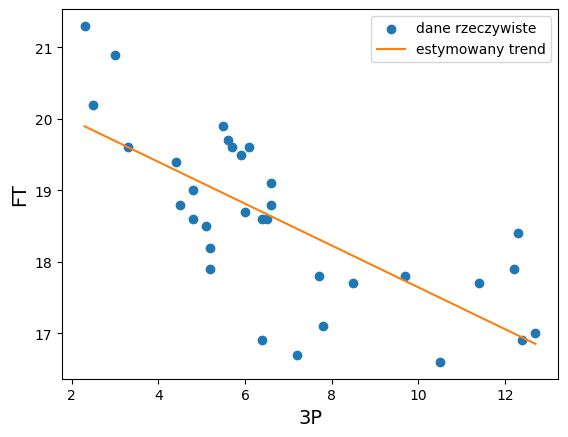
\includegraphics[width=10cm]{wykres_zaleznosci_FT_od_3P.png}
                \caption{Zależność liczby udanych rzutów osobistych od liczby udanych rzutów za 3 punkty}
                \label{fig:wykres_zaleznosci_FT_od_3P}
            \end{figure}

        Wraz ze wzrostem liczby udanych rzutów za 3 punkty, liniowo maleje liczba udanych rzutów osobistych. Rzuty osobiste wynikają bezpośrednio z nieprzepisowego zatrzymania zawodnika podczas rzutu, co zdarza się znacznie częściej przy rzutach za 2, niż za 3 punkty.  

            
    

         \item Podsumowanie:
         
         Stopień dopasowanego trendu wybierany był na podstawie obserwacji. Dosyć   istotnym problemem, napotkanym przy próbach estymacji trendu było to, że danych było stosunkowo mało oraz znajdowały się na one naprawdę małym wycinku, co w większości prowadziło do zauważalnie sporych przekłamań w wyrazie wolny wielomianów lub powodowało gwałtowne dążenie funkcji do nieskończoności.

        Prawie wszystkie silne korelacje okazywały się liniowe. Spora liczba statystyk bezpośrednio z siebie wynika, jak np. PTS i FG. Silne korelacje dodatnie wykazywały ze sobą również statystyki, które na przestrzeni lat zmieniły się w ten sam sposób np. BLK i STL, lub w przypadku silnych korelacji ujemnych w sposób przeciwny. Jedynym wyjątkiem od tej reguły jest kwadratowa zależność liczby punktów od liczby udanych rzutów za 3 punkty. W tym przypadku liczba udanych rzutów za 3, z każdym sezonem, zaliczała wzrost, a liczba punktów wpierw malała, a następnie rosła.

    \end{enumerate}

\section{Modelowanie}

    \subsection{Przygotowanie danych}

    Zbiór "Per Game Stats" podzielony został na dane treningowe i dane testowe, w sposób losowy, w stosunku 80/20. Następnie kolumny tego zbioru zostały podzielone na cechy numeryczne (FG, 3P, FT, TRB, AST, STL, BLK, TOV, PF, PTS) i kategoryczne (Season). W przypadku braku występowania któreś z danych w wierszu, jeżeli była ona wartością numeryczną, wstawiana była wartość średnia danej kolumny. W przypadku braku wartości kategorycznej wstawiana była najczęściej występująca kategoria. Do przekształcania cech numerycznych użyty został również scaler, który pomógł wyrównać skale tych cech. Z kolei przy przekształcaniu cech kategoryczny zastosowano encoder, który utworzył dodatkowe kolumny z każdą unikalną wartością cechy kategorycznej. 
    Modele otrzymały dane treningowe z 421 wierszami należącymi do klasy dostającej się do fazy play-off i 351 do klasy nie grającej w daleszej części sezonu. W danych testowych znalazło się 111 wierszy ze statystykami pozwalającymi na awans do fazy play-off i 83 wierszy ze statystykami nie dającymi gry w fazie play-off. Większa ilość wierszy klasy dostającej się do fazy play-off, wynika z faktu, iż w każdym sezonie do 2020-21, do fazy tej awansowało 16 drużyn, a analizowane sezony posiadały od 27 do 30 drużyn. W sezonach 2019-20, 2020-21, 2021-22 oraz 2022-23 wprowadzono turniej play-in, do którego awans traktowany jest w badaniu, jak awans do play-off, co zwiększyło liczbę awansujących drużyn z 16 do 18 w sezonie 2019-20 i do 20 w pozostałych sezonach.
    Do stworzenia modeli wykorzystano bibliotekę sklearn.


    \subsection{Dobór modelu}
    \begin{enumerate}
    \item \textbf{Model KNN}
    \begin{enumerate}
        \item Przygotowanie modelu

        Do utworzenia modelu zastosowana została metryka cosinusowa, a ilość sąsiadów została ustawiona na 14.
        
        \item Test modelu
        \begin{table}[H]
            \centering
            \begin{tabular}{|l|l|l|}
            \hline
             & \textbf{YES (actual)} & \textbf{NO (actual)}  \\ \hline
            \textbf{YES (predicted)} & 84 & 24 \\ \hline
            \textbf{NO (predicted)} & 27 & 59  \\ \hline
            \end{tabular}
        \end{table}
 \newpage        
        \begin{table}[H]
            \centering
            \begin{tabular}{|l|l|l|l|}
            \hline
            & \textbf{precision} & \textbf{recall} & \textbf{f1-score}  \\ \hline
            \textbf{NO} & 0.69 & 0.71 & 0.70 \\ \hline
            \textbf{YES} & 0.78 & 0.76 & 0.77 \\ \hline
            \textbf{macro avg} & 0.73 & 0.73 & 0.73 \\ \hline
            \textbf{weighted avg} & 0.74 & 0.74 & 0.74 \\ \hline
            \end{tabular}
        \end{table}
        Dokładność modelu: 0.74
        \item Analiza modelu
        
        Łącznie 143 wiersze zostały przewidzianych prawidłowo i 51 błędnie. Model dał dosyć wysoką dokładność, ponieważ jest w stanie przewidzieć bliko 3/4 wierszy ze statystykami. Lepiej poradził sobie z przewidywaniem statystyk pozwalającymi na grę w fazie play-off, co wynika z precyzji predykcji klasy "YES" większej o 0.09. Jednak różnica nie była już tak znacząca w przypadku recall, gdzie zmniejszyła się ona do 0.05.
    \end{enumerate}

    \item \textbf{Model SVC}
    \begin{enumerate}
        \item Przygotowanie modelu

        Do utworzenia modelu zastosowane zostało jądro rbf. 
        
        \item Test modelu

        \begin{table}[H]
            \centering
            \begin{tabular}{|l|l|l|}
            \hline
             & \textbf{YES (actual)} & \textbf{NO (actual)}  \\ \hline
            \textbf{YES (predicted)} & 95 & 31 \\ \hline
            \textbf{NO (predicted)} & 16 & 52  \\ \hline
            \end{tabular}
        \end{table}
        
        \begin{table}[H]
            \centering
            \begin{tabular}{|l|l|l|l|}
            \hline
            & \textbf{precision} & \textbf{recall} & \textbf{f1-score}  \\ \hline
            \textbf{NO} & 0.76 & 0.63 & 0.69 \\ \hline
            \textbf{YES} & 0.75 & 0.86 & 0.80 \\ \hline
            \textbf{macro avg} & 0.76 & 0.74 & 0.75 \\ \hline
            \textbf{weighted avg} & 0.76 & 0.76 & 0.75 \\ \hline
            \end{tabular}
        \end{table}
        Dokładność modelu: 0.76
        \item Analiza modelu
        
        Łącznie 147 wierszy zostało przewidzianych prawidłowo i 47 błędnie. Model dał nam wysoką dokładność, przewidując ponad 3/4 wierszy prawidłowo. Sklasyfikował zdecydowanie większą ilość wierszy jako posiadające odpowiednie statystyki, aby dostać się do fazy play-off. Stosunek przewidzianych wystąpień klasy "YES" do "NO" wyniósł 126/68, przy rzeczywistym 111/83. Poskutkowało to wysokim recallem klasy, dostającej się do fazy play-off (0.83) i ewidentnie niższym klasy kończącej rozgrywki (0.63). Precyzja przewidywania obu cech różniła się nieznacznie.
        

        
    \end{enumerate}

    \item \textbf{Model DecisionTree}
    \begin{enumerate}
        \item Przygotowanie modelu

        Zastosowano domyślne parametry modelu.
        
        \item Test modelu

        \begin{table}[H]
            \centering
            \begin{tabular}{|l|l|l|}
            \hline
             & \textbf{YES (actual)} & \textbf{NO (actual)}  \\ \hline
            \textbf{YES (predicted)} & 79 & 27 \\ \hline
            \textbf{NO (predicted)} & 32 & 56  \\ \hline
            \end{tabular}
        \end{table}

        
        \begin{table}[H]
            \centering
            \begin{tabular}{|l|l|l|l|}
            \hline
            & \textbf{precision} & \textbf{recall} & \textbf{f1-score}  \\ \hline
            \textbf{NO} & 0.65 & 0.66 & 0.65 \\ \hline
            \textbf{YES} & 0.74 & 0.73 & 0.74 \\ \hline
            \textbf{macro avg} & 0.70 & 0.70 & 0.70 \\ \hline
            \textbf{weighted avg} & 0.70 & 0.70 & 0.70 \\ \hline
            \end{tabular}
        \end{table}

        Dokładność modelu: 0.70
        \item Ważność atrybutów
        \begin{table}[H]
            \centering
            \begin{tabular}{|l|l|}
            \hline
            \textbf{Cecha} & \textbf{Ważność}  \\ \hline
            TOV & 0.1659 \\ \hline
            FT & 0.1312 \\ \hline
            AST & 0.1106 \\ \hline
            TRB & 0.0998 \\ \hline
            PF & 0.0992 \\ \hline
            STL & 0.091 \\ \hline
            FG & 0.0795 \\ \hline
            BLK & 0.076 \\ \hline
            3P & 0.0478 \\ \hline
            Season 2006-07 & 0.0158 \\ \hline
            Season 2013-14 & 0.0141 \\ \hline
            PTS & 0.0114 \\ \hline
            Season 1998-99 & 0.011 \\ \hline
            Season 2015-16 & 0.0098 \\ \hline
            Season 1995-96 & 0.0089 \\ \hline
            Season 2022-23 & 0.0049 \\ \hline
            Season 2017-18 & 0.0048 \\ \hline
            Season 2000-01 & 0.0044 \\ \hline
            Season 1999-00 & 0.0041 \\ \hline
            Season 2018-19 & 0.0038 \\ \hline
            Season 2014-15 & 0.0035 \\ \hline
            Season 1994-95 & 0.0014 \\ \hline
            Season 2003-04 & 0.0009 \\ \hline
            
            
            
            \end{tabular}
        \end{table}

        \item Analiza modelu
        Łącznie 147 wierszy zostało przewidzianych prawidłowo i 47 błędnie. Model dał nam dokładność wynoszącą 7/10. Ponownie, model był znacznie bardziej precyzyjny w przypadku przewidywania zespołów, które dostaną się do fazy play-off. Zarówno precyzja i recall różniły się o około 0.09, z przewagą klasy "YES". Najważniejszą cechą, przy przewidywaniu, okazała się liczba strat, liczba udanych rzutów osobistych oraz liczba asyst, a najmniej istotne okazały się liczba rzutów za 3 punkty, liczba punktów oraz informacja o sezonie. Część sezonów zostały określone przez model jako nieistotne, jednak nie została odnaleziona żadna zależność określająca, dlaczego model podjął taką decyzję. 
        
    \end{enumerate}
    

        \item Podsumowanie
        
        Wybory parametrów, przedstawianych modeli, dokonywane były poprzez przeprowadzanie testów na ich różnych kombinacjach i wyborze jednej prowadzącej do największej dokładności.

         Różnice między dokładnością poszczególnych modeli nie okazały się duże. Najdokładniejszy okazał się SVC z dokładnością 0.76, a najmniej dokładny DecisionTree z dokładnością 0.7. Każdy z modeli radził sobie znacznie lepiej z przewidywaniem klasy cech, które dostaną się do fazy play-off, co najprawdopodobniej wynika z minimalnie większej ilości wierszy tej klasy w danych treningowych. Bazując na wynikach dokładności zastosowanych modeli, można uznać, że na podstawie wybranych w tym eksperymencie statystyk oraz wiadomości o sezonie z którego pochodzą, jesteśmy w stanie stworzyć model, który z zadowalającą dokładnością przewiduje, czy drużyna dostałaby się do fazy play-off w podanym sezonie. Wartym spostrzerzenia faktem jest mała istotność cechy związanej z konkretnym sezonem w modelu DecisionTree, a duża związana ze statystykami numerycznymi, zarówno ofensywnymi, jak i defensywnymi.

    \end{enumerate}

    \subsection{Eksperymenty na modelu}

    \begin{enumerate}
        \item Opis eksperymentu
        
        Korzystając z modelu DecisionTree, przeprowadzony został eksperyment, pozwalający ocenić, czy aktualne drużyny NBA prezentują poziom wyższy, czy niższy, niż drużyny z sezonów w poprzednich dekadach. Wybór modelu wynika z największej dokładności, jego predykcji, dotyczącej drużyn z obecnego sezonu w obecnym sezonie, z pośród wszystkich modeli (pozostałe modele przewidywały 24 drużyny z tego sezony jako drużyny, które dostały się do fazy play-off, czyli aż o 4 za dużo) oraz z powodu jawnie znanych i przeanalizowanych wcześniej ważności poszczególnych cech wykorzystywanych przez ten model.
        W pierwszej fazie eksperymentu ze zbioru danych "Per Game Stats", wycięte zostały wiersze dotyczące drużyn jedynie z tego sezonu. Następnie zmieniając ich wartość w kolumnie Season, na wybrany sezon z przeszłości, policzone zostało, ile z nich, model sklasyfikował jako drużyny, które dostałyby się do fazy play-off, w podanym przeszłym sezonie. W drugim kroku, role zostały odwrócone i sprawdzone zostało jak drużyny z przeszłości, poradziłyby sobie w obecnym sezonie.

        \item Eksperyment

        Wyniki drużyn z aktualnego sezonu zasadniczego w poprzednich sezonach.

        \begin{table}[H]
            \centering
            \begin{tabular}{|l|l|l|}
            \hline
            \textbf{Sezon} & \textbf{YES} & \textbf{NO}  \\ \hline
            \textbf{2022-23} & 20 & 10  \\ \hline
            \textbf{2017-18} & 22 & 8  \\ \hline
            \textbf{2012-13} & 22 & 8  \\ \hline
            \textbf{2007-08} & 22 & 8  \\ \hline
            \textbf{2002-03} & 22 & 8  \\ \hline
            \textbf{1997-98} & 22 & 8  \\ \hline
            \textbf{1992-93} & 22 & 8  \\ \hline
            \end{tabular}
        \end{table}

        Wyniki drużyn z poprzednich sezonów w aktualnym sezonie zasadniczym.
        
        \begin{table}[H]
            \centering
            \begin{tabular}{|l|l|l|}
            \hline
            \textbf{Sezon} & \textbf{YES} & \textbf{NO}  \\ \hline
            \textbf{2022-23} & 20 & 10  \\ \hline
            \textbf{2017-18} & 16 & 14  \\ \hline
            \textbf{2012-13} & 13 & 17  \\ \hline
            \textbf{2007-08} & 17 & 13  \\ \hline
            \textbf{2002-03} & 16 & 13  \\ \hline
            \textbf{1997-98} & 15 & 14  \\ \hline
            \textbf{1992-93} & 15 & 12  \\ \hline
            \end{tabular}
        \end{table}

        \item Obserwacje

        Drużyny z aktualnego sezonu poradziły sobie zdecydowanie lepiej, od drużyn z przeszłości. W każdym sezonie, model przewidział, że 22 z nich dostałyby się do fazy play-off, co odpowiada jedynie 8 drużyną, którym by się to nie udało. Warto zwrócić uwagę, że w pozostałych badanych sezonach, limit drużyn awansujących do fazy play-off wynosił 16, w związku z czym, obecne drużyny przekroczyły go w każdym sezonie, aż o 6. W drugiej fazie eksperymentu, zaobserwowano, że drużyny z przeszłości miałyby spore problemy znajdując się w obecnym sezonie. Żadnej z przeszłych ekip nie udało się przebić liczby dwudziestu przechodzących dalej drużyn. Najlepszy wynik osiągnęły drużyny z sezonu 2007-08 (17), a najgorszy 2012-13 (13). Drużyny z lat 90-tych dwukrotnie osiągały przewidywania 15 drużyn dostających się do fazy play-off.
        
    \end{enumerate}
    


\section{Wnioski}

Udało się zrealizować wszystkie cele projektu.

Od początku lat 90-tych, poszczególne statystyki przechodziły różne zmiany. Porównując je bezpośrednio, zauważyć można spadek statystyk defensywnych, takich jak odbiory i bloki. Jednak wraz z nimi spadła ilość popełnianych fauli, która z pewnością wpływa na większe bezpieczeństwo zawodników, co jest niezwykle kluczowe w grze, tak kontaktowej, jak koszykówka. Drużyny osiągają również średnio o 2 straty mniej. Statystyki, które na przestrzeni analizowanych sezonów zmalały i znów wzrosły, również malały najczęściej i najgwałtowniej w latach 90-tych. Oznacza to łącznie 9 na 10 stopniowo zmniejszających się statystyk, co sugeruje, że tamto dzisięciolecie było momentem spadku poziomu NBA. Sytuacja odwraca się dopiero w latach 2010-tych, gdzie statystyki takie jak FG, TRB, AST i PTS znów zaczęły rosnąć. Zmiany wspomnianych statystyk, poza PTS i 3P, jednak nie okazały się duże, co pozwala nam stwierdzić, że mimo postępujących zmian, same fundamenty ligi pozostają niezmienne. Z całej tej analizy wyłamuję się liczba rzutów za 3 punkty, która przez cały analizowany okres, zwiększała się będąc jedyną znacznie zmieniająca sie statystyką.

Badanie korelacji między statystykami potwierdziło wiele zależności oraz zaprezentowało, że statystyki prawie w każdym przypadku wpływają na siebie liniowo, co wynika z bezpośredniego ich wpływu na siebie lub ich podobnie przebiegających zmian na przestrzeni lat. Jedyną statystyką, której wzrost powodował spadek innych statystyk były udane rzuty za 3 punkty, jednak zmiany z jej zwiększaniem się skorelowane nie były znaczne. Kwadratowa zależność liczby punktów na mecz od liczby udanych rzutów za 3 punkty oraz trwający aktualnie wzrost obu tych statystyk, z każdym sezonem, pozwala stwierdzić, że zawodnicy obecnie znacznie bardziej skupiają trening wokół tej umiejętności, co bezpośrednio wpływa na poprawę ofensywy drużyny. Biorąc pod uwagę fakt, iż aktualnie średnia liczba punktów jest prawie o 10 większa niż na początku lat 90-tych i prawie o 20 większa niż pod ich końcówkę, można to określić jako pozytywną zmianę.

Stworzone modele posiadały dokładność w okolicach 0.7 do 0.76, co uznawane jest za wynik satysfakcjonujący. Kluczowa przy analizie zmian jest tabela ważności cech w modelu DecisionTree. Brak lub mała istotność pochodzenia wiersza z poszczególnego sezonu potwierdza, że na przestrzeni sezonów 1990-91 - 2022-23 wartości cech numerycznych nie zmieniły się na tyle drastycznie, aby kluczową informacje stanowił sezon, z którego pochodzą dane. Ku zaskoczeniu, kluczowa przy przewidywaniu klasy modelu okazała się statystyka strat. Wpływ na to może mieć, fakt iż drużyny prowadzące w meczu, szczególnie w końcówce, mają tendencję by rzadziej tracić piłkę i częściej oddawać rzuty osobiste po faulach drużyny przeciwnej. Koniec, końców to procent zwycięstw w sezonie daje awans, a nie liczba punktów.

Wyniki eksperymentu prowadzą do bezpośredniego porównania formy obecnych drużyn, z tymi z przeszłości. Drużyny teraźniejsze poradziły sobie zdecydowanie lepiej w przeszłości niż drużyny przeszłe w teraźniejszości. W latach 90-tych, 22 drużyny awansowałyby do fazy play-off, czyli o dwie więcej niż w przypadku ich gry w sezonie z którego pochodzą. Natomiast dla drużyn z początku i końca lat 90-tych przewidywane jest jedynie 15 miejsc w play-offach 2022-23. Pokazuje to, że aktualne drużyny bezpośrednio radzą sobie lepiej od drużyn z lat 90-tych.

Reasumując, wynik eksperymentu oraz analiza danych wskazuje na wzrost poziomu ligi NBA względem lat 90-tych. Co więcej, poziom ten wykazuje tendencje do ciągłego wzrostu. Statystykami mocno wyróżniającymi się, w porównaniu do sezonów sprzed 30 lat, są jedynie udane rzuty za 3 punkty oraz liczba punktów. Pomimo zmian stylu gry, 8 z 10 analizowanych statystyk nie zmieniły się znacznie. Dodatkowo są to statystyki, uznawane przez model, jako najbardziej kluczowe w predykcji awansu drużyny do fazy play-off, co tym bardziej przeczy teorii mówiącej, że aktualna koszykówka na stadionach NBA niczym nie przypomina lat 90-tych. Zmiany są nieodłączną częścią każdego sportu, a liga NBA nie jest tu wyjątkiem. Jednak w tym przypadku ewolucja nie jest gwałtowna i prowadzi do zwiększenia poziomu rozgrywek, co powinno zostać częściej zauważane i respektowane.




\bibliographystyle{plain}
\bibliography{references}

\begin{thebibliography}{9}
\bibitem{nba_website}
NBA official website. Available: \url{https://www.nba.com/}

\bibitem{basketball_reference}
Basketball-Reference. Available: \url{https://www.basketball-reference.com/}

\end{thebibliography}
\end{document}
